\documentclass[notitlepage]{report}

\usepackage[hyphens,spaces,obeyspaces]{url}
\usepackage{hyperref}
\usepackage{amsfonts}
\usepackage{amsmath}

\renewcommand\thesection{\arabic{section}}
\renewcommand\thechapter{\arabic{chapter}}

\usepackage{etoolbox}
\patchcmd{\thebibliography}{\chapter*}{\section*}{}{}
\renewcommand{\bibname}{References}

\usepackage{graphicx}
\graphicspath{{../run/}}

\let\vec\mathbf
\newcommand{\matr}[1]{\mathbf{#1}}
\begin{document}

\begin{titlepage}
\thispagestyle{empty}

\title{Pattern recognition using singular value decomposition}
\author{Daniel Holmberg}
\maketitle

\vfill

\begin{abstract}
This paper presents a linear algebra method for pattern recognition. Singular value decomposition is used to distinguish single handwritten digits. I implement a method for giving test images to the program and examine the goodness of recognition when accounting for different number of variations in the training data.
\end{abstract}

\vfill

\renewcommand{\chapter}[2]{}
\tableofcontents

\vfill

\end{titlepage}

\section{Introduction}
Singular value decomposition (SVD) of matrices can be used for recognizing simple patterns. I will present some theory and my implementation of the method. It needs a training set of in my case handwritten digits in the interval 0 to 9. These were obtained from the NIST database \cite{nistdata} and has been converted to MATLAB format \cite{helsinkidata} using the script from ref. \cite{converted}. The variation within each digit's set is modeled using an orthogonal basis in the digits' image space. This basis comes from the SVD.

By computing the relative residual of an arbitrary handwritten number in each of the ten digits' bases we can decide which one of them it is. Namely most likely the one with the smallest residual as long as it looks somewhat alike to the training data. I made the code so that it is possible to try a random number in the NIST test database as well as giving the program more of a challenge by inputting your own images of handwritten digits.

\newpage

\section{Methods}
The training set of images are $m_{\textrm{im}} \times m_{\textrm{im}} = m$ matrices where $m_{\textrm{im}} = 28$ in the NIST data, thus $m = 784$. Each image $a_i$ is a column in the matrix $A$ spanning the subspace $\mathbb{R}^m$ so that the complete training data becomes $A\in \mathbb{R}^{m \times n}$ where $n$ is the number of images. The SVD is used to get an orthogonal basis of the image subspace so that variations within the set of training digits can be modeled. A can be written using the SVD as
\begin{equation}
\matr{A} = \matr{U} \matr{\Sigma} \matr{V}^\textrm{T}
\end{equation}
where $U\in \mathbb{R}^{m \times m}$ is unitary, $\Sigma\in \mathbb{R}^{m \times n}$ is diagonal and $V\in \mathbb{R}^{n \times n}$ is also unitary. The training images can then be approximated using the $k$ most dominant singular values $\sigma$ which are the diagonal entries of the matrix $\Sigma$
\begin{equation}
\matr{A} \approx \sum_{i=1}^k \sigma_i \vec{u}_i \vec{v}_i^\textrm{T}
\end{equation}
If we reshape the vectors $u_i$ back to images the first singular vector represent the number while the following singular images should represent the dominating variations of that digit's the training set. So the basis in which an unknown digit can be best approximated in is likely what that digit is. An arbitrary image can be approximately expressed in the U basis as
\begin{equation}
\vec{z} = \sum_{i=1}^k \alpha \vec{u}_i = \matr{U}_k\vec{\alpha}
\end{equation}
and the coefficients $\alpha_i$ can be obtained by computing the residual vector in a least squares problems
\begin{equation}
\min_{\alpha_i} || \vec{z}-\sum_{i=1}^k \alpha \vec{u}_i||
\end{equation}
which can be written using the Euclidean norm as
\begin{equation}
\label{min}
\min_{\vec{\alpha}} || \vec{z}-\matr{U}_k \vec{\alpha}||_2
\end{equation}
Since U is unitary the columns form a set of orthonormal vectors and the solution to \eqref{min} is given by $\alpha = U_k^\textrm{T} z$. The norm of the residual vector of the least squares problem is
\begin{equation}
||(\matr{I} - \matr{U}_k \matr{U}_k^T)\vec{z}||_2
\end{equation}
and what I calculate is the relative residual
\begin{equation}
\label{res}
r = ||(\matr{I} - \matr{U}_k \matr{U}_k^\textrm{T})\vec{z}||_2/||\vec{z}||_2
\end{equation}
which ranges from 0 to 1. The lower the value the better is the match of test digit compared to the training digits. \cite{eldén_2006}

\newpage

\section{Implementation}

I implemented the theory as an algorithm that starts by computing the SVD of each set of digit training data. This is done by \verb|svd()| in MATLAB. I then compare the relative residual between all ten digits' bases, each with k basis vectors as that is the cut-off parameter in \eqref{res}. The program classifies the input as the digit in the training data that yields the smallest relative residual. 

The training data is for some reason flipped left to right and rotated counterclockwise so I have to replicate that when testing an image \\
\verb|z = rot90(fliplr(reshape(z, 28, 28)))|. Then at the heart of the program lies the calculation of the residual and that can be written as a one-liner:\\ 
\verb|r = norm((eye(784, 784) - U(:, 1:k)*U(:, 1:k)')*z)/norm(z)|.

This program is executed by opening the \textit{src} folder in MATLAB and running \textit{main.m} by pressing run or typing main in the MATLAB command window. The program can do two things, either graph relative residual values up to a given value k, or try to identify a digit. It can work with images which must be placed in the \textit{run} folder and the requirements for them are that they must be square shaped, have a white (rgb: [255, 255, 255]) background and the digit itself is black (rgb: [0, 0, 0]). There are three examples in the run folder of different size. Other than that the program gives you the option to test an arbitrary image from the test file \textit{src/testdata/t10k-images-idx3-ubyte.gz} \cite{nistdata}. The test digits are converted using \textit{src/testdata/loadmnist.m} \cite{loadmnist}.

All of my test images are recognized correctly by the program even at low values of k. For example to test it for the digit seven, first open \textit{src} as current folder and then run the program:
\begin{verbatim}
>> cd [your-path-to-svd]/SVD-pattern-recognition-master/src/
\end{verbatim}
\begin{verbatim}
>> main
Welcome! This is the pattern recignition bot beep boop
------------------------------------------------------
Write "test" for testing one number or "graph" for data collection: test
Filename of your digit image or "r" for a random number: image7.png
Integer value for cut-off parameter k: 10
Relative residual = 0.61982
Predicted number = 7
\end{verbatim}
This will also display how the number is interpreted as by my code. You can play around by running multiple times and typing "r" instead of a filename or testing different values of k.

A graph can be plotted for a given image file like this:
\begin{verbatim}
Welcome! This is the pattern recignition bot beep boop
------------------------------------------------------
Write "test" for testing one number or "graph" for data collection: graph
Filename of your digit image: image3.png
Integer value for cut-off parameter k: 30
\end{verbatim}
These graphs are presented in the result section.

\newpage

\section{Results}
When graphing over many $k$ the residual of an image a variable $y$ is created in the workspace. This has as it first row what numbers the images has been recognized as. The indices of $y$ represent $k$ and there are $k+1$ of the since I wanted to start from 0 as a reference point and go up to the given number. The relative residual will always be $1$ and the digit can not be recognized at $k=0$. 

I made plots up to $k=30$ for each of my three test images to see how the residual behaves. My digits was interpreted correctly from the start with very low $k$ values, I checked that in the $y$ array. The only instance where it did not work in the interval $k\in[1, 30]$ was for \textit{image3.png} for $k=26$ where it apparently resembles a $2$ more. Just for fun I checked for much higher numbers and my digit 3 stops being recognized correctly at $k=82$. Since the higher the number the more variations in the training set are accounted for and not just the really important dominating ones, it will become just a blur and really arbitrary what the input is classified as.

My smallest one, \textit{image3.png} is only $28$ by $28$ pixels which is exactly as big as the training data images are. My code does therefore not scale it, only inverts the color (fig \ref{out3}) to match the white on black NIST data. Its relative residual gradually decreases as it should in graph \ref{graph3}.
\begin{figure}[!ht]
\centering
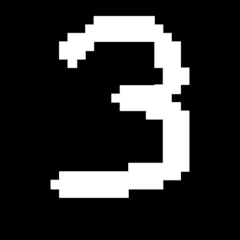
\includegraphics[scale=0.25]{output3.png}
\caption{Interpreted version of image3.png}
\label{out3}
\end{figure}

\begin{figure}[!ht]
\centering
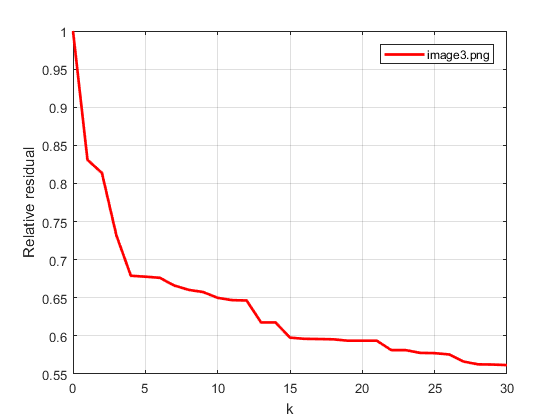
\includegraphics[scale=0.575]{image3graph.png}
\caption{Relative residual for image3.png for different number o basis vectors}
\label{graph3}
\end{figure}

My middle sized one is \textit{image7.png} which is $240$ by $240$ pixels is interpreted as fig \ref{out7} and the residual behaves as in graph \ref{graph7}.
\begin{figure}[!ht]
\centering
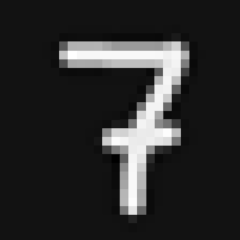
\includegraphics[scale=0.4]{output7.png}
\caption{Interpreted version of image7.png}
\label{out7}
\end{figure}

\begin{figure}[!ht]
\centering
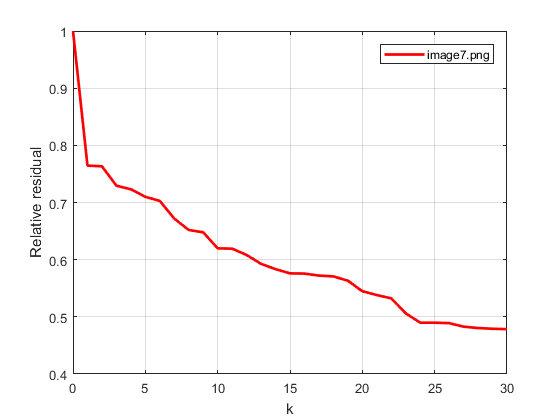
\includegraphics[scale=0.65]{image7graph.png}
\caption{Relative residual for image7.png for different number o basis vectors}
\label{graph7}
\end{figure}

My largest image is \textit{image8.png}, $360$ by $360$ pixels. These last two images not only have their colors inverted but are also scaled to be $28 \times 28$.
\begin{figure}[!ht]
\centering
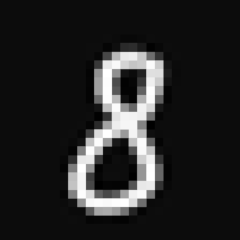
\includegraphics[scale=0.4]{output8.png}
\caption{Interpreted version of image8.png}
\label{out8}
\end{figure}

\begin{figure}[!ht]
\centering
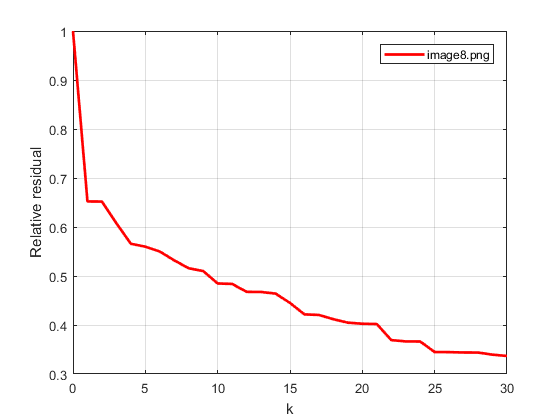
\includegraphics[scale=0.65]{image8graph.png}
\caption{Relative residual for image8.png for different number o basis vectors}
\label{graph8}
\end{figure}

As we can see the relative residual becomes smaller as more variations in the training digits are taken into account as it should. It is also worth noting that the larger the image the faster the relative residual decreases. This means that my larger images seven \ref{out7} and eight \ref{out8} are interpreted by the code to be more alike the training data than my number 3 (image \ref{out3}). That is certainly because the training digits are also smooth from the beginning and gets pixelated in the same way as my larger images. My \textit{image7.png} might also get somewhat worse result since everybody does not write it with a horizontal line crossing in the middle.

Timewise the program works very fast when the training data has been calculated, and it will only do that once. The training data takes about 30 seconds to finish and is saved in the workspace as a variable U. The program can then almost instantaneously recognize test digits.

\newpage

\section{Conclusions}
This method works well for identifying digits. It is a good and fast method to apply when the image you want identified is simple and easily distinguishable from the other alternatives, other than digits are letters the first that come to mind. This method seem kind of ideal for a fairly low number $k$ of basis vectors, it never failed me for values of around 5-20. It is important that the input looks like the training data, that is why if you run with a random number from the NIST test database it will almost always be recognized correctly depending on you value of $k$. 

Give it a try by drawing a digit with black on a white square background in Paint or something. Then place it in the run folder and give it as input to the program and see how it goes...
\bibliography{sources}
\bibliographystyle{ieeetr}

\end{document}
